\begin{chapter}{Der Beweis von Robertson, Sanders, Seymour und Thomas}
  Die Grundidee des Beweises besteht darin, eine bestimmte Menge von 633 sogenannten Konfigurationen -- welche nicht mit den Konfigurationen von Appel \& Haken zu verwechseln sind -- aufzustellen und dann zu zeigen, dass kein Element dieser Menge in einem minimalen Gegenbeispiel vorkommen kann -- dieser erste Schritt wird \textit{Reduzierbarkeit} (engl.: reducibility) genannt. Damit folgt der Beweis der Idee seiner Vorgänger, allerdings mit dem Unterschied, dass jedes minimale Gegenbeispiel eine \textit{intern 6-fach zusammenhängende Triangulation} ist. \\
  Im zweiten Schritt wird gezeigt, dass in jeder intern 6-fach zusammenhängenden Triangulation eine der oben genannten Konfigurationen vorkommen muss -- auch \textit{Zwangsläufigkeit} (eng.: unavoidability) genannt. Zusammen zeigt dies, dass es kein minimales Gegenbeispiel geben kann und der Vierfarbensatz somit wahr ist. \\
  Der wesentliche Unterschied zum vorher vorgestellten Beweis von Appel \& Haken liegt darin, auf welche Art die Zwangsläufigkeit hergestellt wird.
  
  \begin{section}{Konfigurationen}
 Ein minimales Gegenbeispiel ist ein planarer Graph $G$, der nicht 4-färbbar ist, derart dass aber jeder planare Graph $G'$ mit $|V(G')| + |E(G')| < |V(G)| + |E(G)|$ eine gültige 4-Färbung besitzt. Unser Ziel ist also, zu zeigen, dass es keinen solchen Graphen $G$ geben kann. 
   
 Aus den allgemeinen Vorüberlegungen wissen wir, dass jedes minimale Gegenbeispiel nur Knoten mit Grad mindestens fünf hat. So sieht man leicht, dass jedes minimale Gegenbeispiel 5-fach knotenzusammenhängend ist. Wir nennen einen Kreis $C$ in einer Triangulation mit fünf oder weniger Knoten einen \textit{Kurzkreis} (engl.: short circuit), wenn sowohl Knoten im inneren Bereich $I$ als auch im äußeren Bereich $O$ von $C$ liegen und wenn für genau fünf Knoten sowohl $I$ als auch in $O$ mindestens zwei Knoten liegen. Wir nennen eine 6-fach knotenzusammenhängende Triangulation \textit{intern 6-fach zusammenhängend}, wenn sie keine Kurzkreise beinhaltet. Das führt zu folgendem Resultat:
  
 \begin{satzl}{}{2.1}
  Jedes minimale Gegenbeispiel ist eine intern 6-fach zusammenhängende Triangulation. 
 \end{satzl}

 Um genauer zu verstehen, warum der Graph 6-fach zusammenhängend sein muss, empfiehlt sich die Lektüre von \cite{AmJMath35}. Birkhoff schaffte es bereits 1913 zu zeigen, dass schwächer zusammenhängende Konfigurationen 4-färbbar sind. Dazu bediente er sich der Resultate von A. B. Kempe -- Ketten, die mit einer beschränkten Auswahl an Farben färbbar sind, und Ringen, die eine Karte in eine innere und eine äußere Region teilen. 
 
 Später werden wir einen Algorithmus kennenlernen, der eine Färbung für eine Triangulation mit Kurzkreis liefert. Daraus lässt sich dann auch der Beweis für Satz \ref{2.1} ableiten.
 
 Als nächstes folgt eine Definition, die fundamental für unseren Beweis ist. Der Begriff der Konfiguration taucht ebenfalls bei Appel \& Haken auf, jedoch besitzt eine Konfiguration dort andere Eigenschaften.
  
 \begin{definition}{Konfiguration}
  Eine Konfiguration $K$ besteht aus einer Beinahe-Triangulation $G(K)$ und einer Zuordnung $\gamma_K : V(G(K)) \mapsto \mathbb{Z}_+$ mit folgenden Eigenschaften:
  \begin{enumerate}[i)]
   \item Für jeden Knoten $v$ besteht $G(K) \setminus \{v\}$ aus höchstens zwei Zusammenhangskomponenten. Gibt es genau zwei, so ist $\gamma_K(v) = d_G(v) + 2$.
   \item Für jeden Knoten $v$, der nicht zur Außenfacette inzident ist, gilt $\gamma_K(v) = d_G(v)$. Für die anderen Knoten $v'$ gilt $\gamma_K(v') > d_G(v')$. In beiden Fällen gilt zusätzlich $\gamma_K(v) \geq 5$.
   \item $K$ hat Ringgröße $\geq 2$. Die \textit{Ringgröße} von $K$ ist definiert als $\sum_v (\gamma_K(v) - d_G(v) - 1)$ für alle Knoten $v$, die zur Außenfacette inzident sind und für die $G(K) \setminus \{v\}$ zusammenhängend ist.
  \end{enumerate}
 \end{definition}
 
 Um $\gamma_K$ für jeden Knoten in einer planaren Zeichnung von $G$ darzustellen, gibt es mehrere Möglichkeiten. Die Offensichtliche wäre natürlich, neben jedem Knoten seinen Wert zu notieren, was jedoch sehr schnell unübersichtlich wird. Stattdessen werden wir unseren Knoten verschiedene Formen geben, wie der folgenden Übersicht zu entnehmen ist.
 
 \[ \begin{tikzpicture}
    \tikzstyle{ann} = [draw=none,fill=none,right]
    \matrix[nodes={draw},column sep=0.5cm] {
    \node[circle,fill=black,inner sep=2pt] {}; &
    \node[draw=none,fill=none] {$\gamma_K(v) = 5$}; \\
    \node[circle,fill=black,inner sep=0.1pt] {}; &
    \node[draw=none,fill=none] {$\gamma_K(v) = 6$}; \\
    \node[circle,inner sep=2pt] {}; &
    \node[draw=none,fill=none] {$\gamma_K(v) = 7$}; \\
    \node[rectangle,inner sep=2.5pt] {}; &
    \node[draw=none,fill=none] {$\gamma_K(v) = 8$}; \\
    \node[regular polygon,regular polygon sides=3,inner sep=1.5pt] {};&
    \node[draw=none,fill=none] {$\gamma_K(v) = 9$}; \\
    \node[regular polygon,regular polygon sides=5,inner sep=2pt] {};&
    \node[draw=none,fill=none] {$\gamma_K(v) = 10$}; \\
    };
\end{tikzpicture}\]
 
 Später werden wir eine Menge aus 633 Konfigurationen betrachten, die für diesen Beweis essenziell sind. Eine vollständige Abbildungsliste findet sich in \cite[Seite 35]{FourRSST}. 
 
 \begin{definition}{Isomorphe Konfigurationen, gute Konfigurationen, auftretende Konfigurationen}
 \-\ 
  \begin{itemize}
   \item Zwei Konfigurationen $K$ und $L$ heißen \textit{isomorph}, falls ein Homeomorphismus der Ebene existiert, der $G(K)$ auf $G(L)$ und $\gamma_K$ auf $\gamma_L$ abbildet. 
   \item Jede Konfiguration, die zu einer der 633 Konfigurationen aus \cite{FourRSST} isomorph ist, bezeichnen wir als \textit{gut}. 
   \item Sei $T$ eine Triangulation. Eine Konfiguration $K$ \textit{tritt in $T$ auf}, wenn $G(K)$ ein Teilgraph von $T$ ist, jede Innenfacette von $G(K)$ eine Innenfacette von $T$ ist und $\gamma_K(v) = d_T(v)$ für alle Knoten von $G(K)$ gilt.
  \end{itemize}

 \end{definition}

   
 Um zu zeigen, dass das eigentliche Problem stets lösbar ist, teilen wir die Suche nach einem minimalen Gegenbeispiel weiter auf. Somit ergeben sich diese beiden Aussagen:
   
 \begin{satzl}{Reduktion}{2.2}
  Wenn eine Triangulation $T$ ein minimales Gegenbeispiel ist, enthält $T$ keine gute Konfiguration.
 \end{satzl}
   
 \begin{satzl}{Zwangsläufigkeit}{2.3}
  In jeder intern 6-fach zusammenhängenden Triangulation $T$ lässt sich eine gute Konfiguration finden.
 \end{satzl}
   
 Kombiniert man die Aussagen der Sätze \ref{2.1}, \ref{2.2} und \ref{2.3}, so sieht man, dass es kein minimales Gegenbeispiel geben kann und damit der Vier-Farben-Satz wahr seien muss. Auf \ref{2.2} werden wir im nächsten Abschnitt genauer eingehen, gefolgt von einem Abschnitt über \ref{2.3}. 
 
 Ein anderer Ansatz, sich der 4-Färbung von Graphen zu nähern, liegt darin, die Facetten auf Färbbarkeit zu untersuchen. Da in einem minimalen Gegenbeispiel jede Innenfacette ein Dreieck ist, benötigen wir eine neue Definiton:
 
 \begin{definition}{Trifärbung}
  Sei $G$ eine Triangulation oder Beinahe-Triangulation, $\kappa:E(G) \mapsto \{-1,0,1\}$ eine Funktion und $r=\{r,f,g\} \subset E(G)$ ein Dreieck. Man sagt, $r$ wird von $\kappa$ \textit{trigefärbt} (engl.: tri-coloured), wenn $\{\kappa(e),\kappa(f),\kappa(g)\} = \{-1,0,1\}$ gilt. Wir sagen, $\kappa$ ist eine \textit{Trifärbung} von $G$, wenn jede Facette von $G$ trifärbbar ist -- oder nur jede Innenfacette, falls $G$ nur eine Beinahe-Triangulation ist.
 \end{definition}

 Statt wie Üblich für die Farben der Facetten $1,2,3$ zu wählen, benutzen wir hier $-1,0,1$, um möglichst nahe am Algorithmus für \ref{2.1} zu bleiben.
 
 \begin{satzl}{Trifärbung $\Leftrightarrow$ 4-Färbung}{tait}
  Eine Triangulation $T$ ist genau dann 4-färbbar, wenn eine Trifärbung ihrer Facetten existiert.
 \end{satzl}
 
 Dass dies tatsächlich der Wahrheit entspricht, wurde bereits von Tait gezeigt, der Beweis ist \cite{TaitTri} zu entnehmen. Der Grund, auf die Färbung von Facetten zu wechseln liegt tatsächlich auch darin, dass ein Algorithmus, der eine Trifärbung bestimmt, leichter zu implementieren war. \cite[Seite 7]{FourRSST} 
 
 Um \ref{2.2} zu beweisen, werden wir für jede Triangulation $T$, die ein minimales Gegenbeispiel sein soll, eine nichtleere Teilmenge der Kanten von $T$ wählen und diese kontrahieren um so eine Darstellung $T'$ zu erhalten. Da $T'$ echt kleiner als $T$ ist, ist diese somit 4-färbbar. Diese Färbung werden wir dann dazu benutzen, eine Färbung für $T$ zu konstruieren, sodass $T$ kein minimales Gegenbeispiel gewesen sein kann. Kontrahiert man Kanten in einem Graphen, ergeben sich verschiedene Notationsprobleme, etwa ob nach der Kontraktion eine nichtkontrahierte Kante im ursprünglichen Graphen immernoch die gleiche Kante wie in der Kontraktion ist. Um die Notationsprobleme um umgehen und die wesentlichen Schwierigkeiten nicht aus den Augen zu verlieren, brechen wir den Kontraktionsprozess in zwei Teile auf. 
 
 \begin{definition}{Zerstreute Menge, Trifärbung modulo $X$}
 Sei $G$ ein Triangulation oder Beinahe-Triangulation. 
 \begin{itemize}
  \item Eine Teilmenge $X \subseteq E(G)$ heißt \textit{zerstreut} (engl.: sparse), wenn jede Innenfacette von $G$ zu höchstens einer Kante aus $X$ inzident und im Falle einer Beinahe-Triangulation die Außenfacette zu keiner Kante inzident ist.
  \item Wenn $X \subseteq E(G)$ zerstreut ist, ist eine \textit{Trifärbung von $G$ modulo $X$} eine Abbildung $\kappa: E(G) \setminus X \mapsto \{-1,0,1\}$ derart, dass für jede Facette von $G$ (außer der Außenfacette bei Beinahe-Triangulationen), die zu den Kanten $e,f,g$ inzident ist, gilt:
  \begin{enumerate}[(i)]
   \item $\{\kappa(e),\kappa(f),\kappa(g)\} = \{-1,0,1\}$, falls $e,f,g \not\in X$
   \item $\kappa(e) = \kappa(f)$, falls $g\in X$.
  \end{enumerate}
 \end{itemize}
 \end{definition}
 
 Dieser Definition folgend ist eine Trifärbung gleichbedeutend mit einer Trifärbung modulo $\emptyset$. 
 
 \begin{satz}{Existenz einer Trifärbung}
  Sei $T$ ein minimales Gegenbeispiel und sei $X\subseteq E(T)$ zerstreut und nicht leer. Gibt es in $T$ keinen Kreis $C$ mit $|E(C) \setminus X| = 1$, so besitzt $T$ eine Trifärbung modulo $X$.
 \end{satz}
 \begin{proof}
  Sei $F$ die Zeichnung der Knoten $V(T)$ und der Kanten aus $X$. Seien $Z_1,\cdots,Z_k$ die Mengen der Knoten, die zu den $k$ Facetten von $F$ inzident sind. Sei nun $S$ ein Graph mit $V(S) =\{Z_1,\cdots,Z_k\}$ und $E(S) = E(T) \setminus X$. Eine Kante $e \in E(S)$ ist inzident zu  $Z_i$, wenn $e \cap Z_i \neq \emptyset$. Da in $T$ kein Kreis mit $|E(C) \setminus X| = 1$ gibt, ist hat $S$ keine Schleifen. Da $S$ durch Kontraktion aus $T$ entsteht, ist $S$ auch planar. Da $X$ nicht leer ist, gilt weiter $|E(S)| + |V(S)| < |V(T)| + |E(T)|$ und da $T$ ein minimales Gegenbeispiel war, besitzt $S$ deshalb eine 4-Färbung. Somt existiert eine Abbildung $\phi: V(T) \mapsto \{1,2,3,4\}$ mit folgenden Eigenschaften:
  \begin{enumerate}[(i)]
   \item Für $1 \leq i \leq k$ ist $\phi(v)$ konstant für $v \in Z_i$ und
   \item für jede Kante $e=\{u,v\}$ von $T$, $e\not\in X$, gilt $\phi(u) \neq \phi(v)$.
  \end{enumerate}
  Für $e=\{u,v\} \in E(S)$ definieren wir\\
  \[\kappa(e) = \begin{cases}
                -1 &\text{ für } \{\phi(u), \phi(v)\} = \{1,2\}\text{ oder } \{3,4\}\\
                0  &\text{ für } \{\phi(u), \phi(v)\} = \{1,3\}\text{ oder } \{2,4\}\\
                1  &\text{ für } \{\phi(u), \phi(v)\} = \{1,4\}\text{ oder } \{2,3\}  
               \end{cases}\]
  Dann ist $\kappa$ eine Trifärbung von $T$ modulo $X$, denn: Sei $r$ eine Facette von $T$, $e=\{u,v\},f=\{v,w\},g=\{w,u\}$. Sind $e,f,g \not\in X$, so sind $\phi(u),\phi(v),\phi(w)$ alle verschieden, also auch $\{\kappa(e),\kappa(f),\kappa(g)\}=\{-1,0,1\}$. Ist andererseits o.B.d.A. $g\in X$, so gilt $\phi(u) = \phi(w)$ und $\kappa(e)=\kappa(f)$. \cite{FourRSST}
 \end{proof}
\end{section}
  \begin{section}{Reduzierbarkeit}
 Wir wollen konsistente Kantenfärbungen definieren. Dazu beginnen diesen Abschnitt mit den dazu nötigen, hinführenden Definitionen:

 \begin{definition}{Kantenfärbung, Match, signiertes Match, signiertes Matching, $\theta$-Passend}
  Sei $R$ ein Kreis und $\theta \in \{-1,0,1\}$.
  \begin{itemize}
   \item Eine \textit{Kantenfärbung} von $R$ ist eine Abbildung $\kappa: E(R) \mapsto \{-1,0,1\}$.
   \item Ein \textit{Match} $m$ ist eine Menge von verschiedenen Kanten $\{e,f\}$ aus $R$. 
   \item Ein \textit{signiertes Match} (engl.: signed match) $(m,\mu)$ ist ein Paar aus einem Match $m$ und $\mu = \pm 1$.
   \item Ein \textit{signiertes Matching} ist eine Menge $M$ von signierten Matches, sodass für unterschiedliche $(\{e,f\},\mu),(\{e',f'\},\mu') \in M$ gilt:
   \begin{enumerate}[(i)]
    \item $\{e,f\}\cap\{e',f'\} = \emptyset$ und
    \item nach dem Löschen von $e'$ und $f'$ liegen $e$ und $f$ in der gleichen Zusammenhangskomponente von $R$.
   \end{enumerate}
   Ist $M$ ein signiertes Matching, so ist $E(M) := \{e\in E(R) | e\in m $ für ein $(m,\mu) \in M\}$.
   \item Eine Kantenfärbung $\kappa$ von $R$ heißt \textit{$\theta$-passend} für ein signiertes Matching $M$ in $R$, wenn gilt:
   \begin{enumerate}[(i)]
    \item $E(M) = \{e \in E(R) | \kappa(e) \neq \theta\}$ und
    \item für alle $(\{e,f\},\mu) \in M$ gilt: $\kappa(e) = \kappa(f) \Leftrightarrow \mu = 1$.
   \end{enumerate}
  \end{itemize}
 \end{definition}
 
 Nun können wir die eigentlich gesuchte Definition aufstellen.
  
 \begin{definition}{konsistente Kantenfärbung}
  Sei $K$ ein Kreis und $\theta \in \{-1,0,1\}$. Eine Menge $\mathscr{C}$ von Kantenfärbungen von $K$ heißt \textit{konsistent}, wenn für jedes $\kappa \in \mathscr{C}$ und jedes mögliche $\theta$ ein signiertes Matching $M$ existiert, so dass $\kappa$ $\theta$-passend für $M$ ist, und $\mathscr{C}$ jede Kantenfärbung, die für $M$ $\theta$-passend ist, enthält.
 \end{definition}

 Für das nächste Teilresultat benötigen wir noch diese Definitionen.
 
 \begin{definition}{Verpackung, Aufzug}
  Sei $H$ eine Beinahe-Triangulation. 
  \begin{itemize}
   \item Dann gibt es einen geschlossenen Pfad $(v_0,v_1,\cdots,v_k)$ durch die zur Außenfacette inzidenten Knoten. Dann existiert ein Kreis $R$ der Länge $k$ mit Kanten $e_1,\cdots e_k$, nicht notwendigerweise ein Kreis in $H$. Für $i \leq i \leq k$ definieren wir einen Zeiger $\phi(e_i) := f_i$, wobei $f_i$ die Kante zwischen $v_{i-1}$ und $v_i$ aus $H$ ist. Wir sagen dann, $\phi$ \textit{verpackt $H$ in $R$}. 
   \item Ist $\kappa$ eine Trifärbung von $H$, so setzen wir für alle $e \in E(R): \lambda(e) = \kappa(\phi(e))$. Dann ist $\lambda$ eine Kantenfärbung von $R$ und wir nennen $\lambda$ einen \textit{Aufzug} von $\kappa$ (durch $\phi$).
  \end{itemize}
 \end{definition}
 
 \begin{satzl}{Konsistente Aufzüge}{3.1}
  Sei $H$ eine Beinahe-Triangulation und $R$ ein Kreis, in den $H$ durch $\phi$ verpackt ist. Sei $\mathscr{C}$ die Menge aller Aufzüge von $\phi$ von Trifärbungen von $H$. Dann ist $\mathscr{C}$ konsistent.
 \end{satzl}
 \begin{proof}
  Sei $e_1,\cdots,e_k$ die Kanten von $R$ und $f_1,\cdots,f_k$ die Kanten des geschlossenen Pfades um die Außenfacette von $H$. Sei $\lambda \in \mathscr{C}$ nud sei $\rho \in \{-1,0,1\}$. Zu zeigen ist, dass ein signiertes Matching $M$ existiert, sodass $\lambda$ $\rho$-passend für $M$ ist, und dass $\mathscr{C}$ alle Kantenfärbungen beinhaltet, sodass $R$ für $M$ $\rho$-passend ist. O.B.d.A. sei $\rho = 0$.\\
  Da $\lambda \in \mathscr{C}$ gilt, ist $\lambda$ der Aufzug einer Trifärbung $\kappa$ von $H$. Eine \textit{Rippe} ist eine Folge $g_0,r_1,g_1,r_2,\cdots,r_t,g_t$, wobei
  \begin{enumerate}[(i)]
   \item $g_0,\cdots,g_t$ verschiedene Kanten von $H$ sind,
   \item $r_1,\cdots,r_t$ verschiede Facetten von $H$ sind,
   \item falls $t >0$ gilt, $g_0$ und $g_t$ beide inzident zur Außenfacette von $H$ sind, oder falls $t=0$ gilt, $g_0$ zu keiner Innenfacette von $H$ inzident ist,
   \item für $1\leq i\leq t$ gilt, dass $r_i$ inzident zu den Facetten $g_{i-1}$ und $g_i$ ist und
   \item für $0\leq i\leq t$ gilt, dass $\kappa(g_i) \neq 0$ gilt.
  \end{enumerate}
  Für jede Rippe sind die Werte von $\kappa(g_0),\cdots,\kappa(g_t)$ abwechselnd $\pm 1$ und für jede Kante $e$, die nicht zur Rippe gehört aber inzident zu einer ihrer Facetten ist, $\kappa(e) = 0$ gilt. Tauscht man die Vorzeichen von $\kappa(g_0),\cdots,\kappa(g_t)$, so erhält man also eine neue Trifärbung von $H$.\\
  Weiter sind alle Rippen disjunkt, sie teilen sich also weder Kanten noch Facetten. Für $1 \leq i \leq k$ lässt sich jede Kante $f_i$ entweder eindeutig einer Rippe zuordnen, wenn $\kappa(f_i) = \pm 1$, oder keiner Rippe zuordnen, wenn $\kappa(f_i)=0$.\\
  Jetzt verknüpfen wir jede Rippe $g_0,r_1,g_1,r_2,\cdots,r_t,g_t$ mit einem signierten Match $(\{e_i,e_j\},\mu)$, wobei $g_0 = f_i$ und $g_t = f_j$ und $\mu = +1$ oder $-1$, je nachdem ob $t$ gerade oder ungerade ist, gilt. Die Menge aller dieser signierten Matches ist ein signiertes Matching $M$ und $\lambda$ ist $\rho$-passend für $M$.\\
  Sei nun $\lambda'$ eine beliebige Kantenfärbung von $R$, die $\rho$-passend für $M$ ist, und definiere $\kappa''(f_i) := \lambda'(e_i)$ (für $1\leq i \leq k$). Dreht man die Vorzeichen von $\kappa$ in einigen Rippen um, so erhält man eine Trifärbung $\kappa'$ von $H$, deren Einschränkung auf $\{f_1,\cdots,f_k\}$ die Trifärbung $\kappa''$ ist. Daraus folgt, dass $\lambda'$ ein Aufzug von $\kappa'$ ist, also wie gefordert $\lambda' \in \mathscr{C}$ gilt. 
 \end{proof}

\begin{definition}{Freie Vervollständigung}
  Sei $K$ eine Konfiguration. Eine Beinahe-Triangulation $S$ heißt \textit{freie Vervollständigung von $K$ mit Ring $R$}, wenn
  \begin{enumerate}[(i)]
   \item $R$ ein induzierter Ring von $S$ ist, der die Außenfacette von $S$ begrenzt,
   \item $G(K)$ ein induzierter Teilgraph von $S$ ist, $G(K) = S \setminus V(R)$ gilt, jede Facette von $G(K)$ auch eine Facette von $S$ ist, die Außenfacette von $G(K)$ den Ring $R$ und die Außenfacette von $S$ beinhaltet,
   \item jeder Knoten $v$ von $S$, der nicht in $V(R)$ liegt, in $S$ Knotengrad $\gamma_K(v)$ hat.
  \end{enumerate}
 \end{definition}
 
 Man kann leicht überprüfen, dass jede Konfiguration eine freie Vervollständigung besitzt. (Hier wird der Umstand benutzt, dass in der Definition von Konfiguration eine Ringgröße $\geq 2$ gefordert ist -- die Ringgröße ist dann genau die Länge des Rings in der Freien Vervollständigung. Gibt es zwei freie Vervollständigungen $S_1$ und $S_2$ von $K$, so existiert ein Homeomorphismus, der $G(K)$ punktweise fixiert und $S_1$ auf $S_2$ abbildet. Dazu verwendet man Eigenschaft (i) aus der Definition der Konfiguration. Es gibt also -- bis auf Isomorphie -- nur eine freie Vervollständigung, weswegen wir von \textit{der} freien Konfiguration sprechen können.
 
 Um die Anschauung des Lesers zu fördern folgt nun die Darstellung einer Konfiguration sowie ihrer freien Vervollständigung. Dabei folgen wir der Notation für die Knoten, wie sie im vorherigen Kapitel dargestellt wurden.
 
 \begin{figure}[hb]
  \label{fig2}
  \[ \begin{tikzpicture}
 \path
    (0,0.5) \blacknode(a1){}
    (0.75,0) \blacknode(b1){} (0.75,1) \blacknode(b2){}
    (1.5,0.5) \smallnode(c1){}
    (2.25,0) \smallnode(d1){} (2.25,1) \smallnode(d2){}        
    (3,0.5) \smallnode(e1){} (3,1.5) \blacknode(e2){};
    \filldraw (a1) -- (b1) -- (c1) -- (d1) -- (e1) -- (e2) -- (d2) -- (c1) -- (b2) -- (a1);
    \filldraw (b1) -- (b2); 
    \filldraw (d1) -- (d2) -- (e1);
\end{tikzpicture} \overset{\overset{\text{freie}}{\text{Vervollständigung}}}{\Longrightarrow} \begin{tikzpicture}
 \path
    (0,1) \blacknode(a1){} (0,2) \blacknode(a2){}
    (0.6,0) \blacknode(x){}
    (0.75,0.5) \blacknode(b1){} (0.75,1.5) \blacknode(b2){} (0.75,2.5) \blacknode(b3){}
    (1.5,0) \blacknode(c1){} (1.5,1) \blacknode(c2){} (1.5,2) \blacknode(c3){} (1.5,3) \blacknode(c4){}
    (2.25,0.5) \blacknode(d1){} (2.25,1.5) \blacknode(d2){} (2.25,2.5) \blacknode(d3){}
    (3,1) \blacknode(e1){} (3,2) \blacknode(e2){}
    (3.75,0.5) \blacknode(f1){} (3.75,1.5) \blacknode(f2){} (3.75,2.5) \blacknode(f3){}
    (4.5,1.5) \blacknode(g1){};
    \filldraw (a1) -- (x) -- (c1) -- (d1) -- (f1) -- (g1) -- (f3) -- (e2) -- (d3) -- (c4) -- (b3) -- (a2) -- (a1) -- (b2) -- (a2);
    \filldraw (x) -- (b1) -- (b2) -- (b3) -- (c3) -- (d2);
    \filldraw (g1) -- (f2);
    \filldraw (e1) -- (e2) -- (f2) -- (e1) -- (d2) -- (e2);
    \filldraw (d3) -- (d2) -- (d1) -- (c2) -- (d2);
    \filldraw (a1) -- (b1) -- (c1) -- (c2) -- (c3) -- (c4);
    \filldraw (d1) -- (e1) -- (f1) -- (f2) -- (f3) -- (d3) -- (c3) -- (b2) -- (c2) -- (b1);
\end{tikzpicture} \]
  \caption[Eine Konfiguration und ihre freie Vervollständigung]{Eine Konfiguration und ihre freie Vervollständigung}
 \end{figure}

 
 \begin{definitionl}{$D$-Reduzibilität}{dred}
  Sei also $S$ die freie Vervollständigung einer Konfiguration $K$ mit Ring $R$. Sei $\mathscr{C}^*$ die Menge aller Kantenfärbungen von $R$ und sei $\mathscr{C} \subseteq \mathscr{C}^*$ die Menge aller Beschränkungen von $E(R)$ von Trifärbungen von $S$. Sei weiter $\mathscr{C}'$ die größte konsistente Teilmenge von $\mathscr{C}^* - \mathscr{C}$. Die Konfiguration $K$ heißt \textit{$D$-reduzibel}, wenn gilt: $\mathscr{C}' = \emptyset$.
 \end{definitionl}
 
 Wir werden später zeigen, dass keine $D$-reduzible Konfiguration in einem minimalen Gegenbeispiel vorkommen kann. In der gängigen Literatur gibt es noch andere Varianten, zu zeigen dass in einem minimalen Gegenbeispiel keine Konfiguration vorkommen kann -- etwa allgemeine $C$-Reduzibilität oder \textit{block count}-Reduzibilität. Für unsere Zwecke benötigen wir zusätzlich lediglich einen Spezialfall der $C$-Reduzibilität.

 \begin{definition}{Zusammenzug}
  Sei $S$ die freie Vervollständigung einer Konfiguration $K$ mit Ring $R$ und sei $\mathscr{C}'$ wie für die $D$-Reduzibilität gewählt. Sei $X \subseteq E(S) - E(R)$. Man sagt, $X$ ist ein \textit{Zusammenzug} (engl.: contract) von $K$, wenn $X$ nicht leer ist, $X$ zerstreut in $S$ ist und keine Kantenfärbung aus $\mathscr{C}'$ die Beschränkung von $E(R)$ einer Trifärbung von $S$ modulo $X$ ist.
 \end{definition}
 
 Eine weitere Bedingung für unsere minimalen Gegenbeispiele ist, dass kein Zusammenzug einer Konfiguration $K$ vorkommen kann. Dies werden wir später weiter ausführen.
 
 Mit Hilfe eines Computers wurde folgendes Resultat von Robertson, Sanders, Seymour und Thomas gezeigt:
 
 \begin{satzl}{Reduzibilität der Konfigurationen}{3.2}
  Für jede der 633 Konfigurationen $K$, die im Anhang (der Originalveröffentlichung) abgebildet sind, sei $X$ die Menge der Kanten, der freien Vervollständigung von $K$, die fett gedruckt sind. Gilt $X \neq \emptyset$, so ist $K$ $D$-reduzibel. Andernfalls gilt $1\leq \sharp X \leq 4$ und $X$ ist ein Zusammenzug für $K$.
 \end{satzl}
 
 Aus diesem Ergebnis werden wir später Satz \ref{2.2} herleiten.

 Selbst wenn $K$ eine Konfiguration ist, die in der Triangulation $T$ auftritt, heißt das noch nicht, dass es eine Teildarstellung von $T$ geben muss, die die freie Vervollständigung von $K$ ist. Dies kann zu Schwierigkeiten führen, wenn wir versuchen, Erkenntnisse über $T$ auf die freie Vervollständigung zu übertragen. 
 
 \begin{definition}{Projektion}
  Sei $T$ eine Triangulation und $S$ eine Beinahe-Triangulation. Eine \textit{Projektion} von $S$ auf $T$ ist eine Abbildung $\phi$ mit Definitionsmenge $D(\phi) = V(S)\cup E(S)\cup F(S)$ derart, dass
  \begin{enumerate}[(i)]
   \item $\phi$ $V(S)$ auf $V(T)$, $E(S)$ auf $E(T)$ und $F(S)$ auf $F(T)$ abbildet,
   \item für verschiedene $u,v \in V(S)$ $\phi(u) = \phi(v) \Leftrightarrow u,v$ beide inzident zur Außenfacette von $S$,
   \item für verschiedene $e,f \in E(S)$ $\phi(e) = \phi(f) \Leftrightarrow e,f$ beide inzident zur Außenfacette von $S$,
   \item für verschiedene $r,s \in F(S)$ $\phi(r) \neq \phi(s)$,
   \item wenn $x,y \in D(\phi)$ inzident in $S$ sind, $\phi(x),\phi(y)$ auch inzident in $T$ sind.
  \end{enumerate}
 \end{definition}
 
 Die folgenden Resultate wollen wir ohne Beweis benutzen, da die Beweise beide langwierig sind und wenig zum Verständnis des eigentlichen Problems beitragen.

 \begin{satzl}{Existenz einer Projektion}{3.3}
  Sei $T$ eine Triangulation und $K$ eine Konfiguration, die in $T$ auftritt. Sei weiter $S$ die freie Vervollständigung von $K$. Dann existiert eine Projektion $\phi$ von $S$ auf $T$ derart, dass $\phi(x) = x$ für alle $x\in V(G(K)) \cup E(G(K)) \cup F(G(K))$. Die Projektion $\phi$ heißt dann auch korrespondierende Projekt.
 \end{satzl}
 
 \begin{satzl}{Darstellung als Beinahe-Triangulation}{3.4}
  Sei $T$ eine Triangulation und $K$ eine Konfiguration, die in $T$ auftritt. Sei $S$ die freie Vervollständigung von $K$ mit Ring $R$. Sei weiter $\phi$ die korrespondierende Projektion von $S$ auf $T$. Sei $H$ die planare Darstellung $T$, die man erhält, wenn man die Knoten aus $V(G(K))$ entfernt, und bezeichne als Außenfacette die Facette von $H$, die $V(G(K))$ enthält. Dann ist $H$ eine Beinahe-Triangulation, und die Einschränkung von $\phi$ auf $E(R)$ verpackt $H$ in $R$.  
 \end{satzl}

 \begin{definition}{Sehen}
  Sei $G$ eine planare Zeichnung eines Graphen. Sei $v \in V(G)$ und $e \in E(G)$. Man sagt $v$ \textit{sieht} $e$, wenn sowohl $v$ als auch $e$ inzident zur gleichen Innenfacette sind, aber $v$ nicht inzident zu $e$ ist.
 \end{definition}

 \begin{definition}{Dreibein}
  Sei $S$ die freie Vervollständigung einer Konfiguration $K$ und sei $X \subseteq E(S)$ zerstreut in $S$ und $\sharp X = 4$. Ein Knoten $v$ aus $S$ heißt \textit{Dreibein} von $X$, wenn gilt:
  \begin{enumerate}[(i)]
   \item $v \in V(G(K))$,
   \item es gibt mindestens drei weitere Knoten in $S$, die zu $v$ adjazent sind und zu Kanten aus $X$ inzident sind und
   \item wenn $\gamma_K(v) = 5$, dann sieht $v$ nicht jede Kante aus $X$.
  \end{enumerate}
 \end{definition}
 
 \begin{satzl}{Existenz eines Kurzkreises}{3.5}
  Sei $T$ eine Triangulation und $K$ eine Konfiguration, die in $T$ auftritt. Sei $S$ die freie Vervollständigung von $K$ und sei $\phi$ die korrespondierende Projektion von $S$ auf $T$. Sei $X \subseteq E(S)$ zerstreut in $S$ und $\sharp X \leq 4$ und wenn $\sharp X = 4$ gilt, so gibt es ein Dreibein für $X$. Gibt es einen Kreis $C$ in $T$ mit $|E(C) - \phi(X)| \leq 1$, so gibt es einen Kurzkreis in $T$.
 \end{satzl}
 \begin{proof}
  Sei $X' = \phi(X) \cap E(C)$. Da $X$ in $S$ zerstreut ist, ist keine Kante aus $X$ inzident zur Außenfacette von $S$. Also ist jede Kante aus $X$ inzident zu zwei verschiedenen Innenfacetten von $S$. Nach Satz \ref{3.3} gilt für jede Facette $t$ von $T$, die zu einer Kante aus $X'$ inzident ist, $t=\phi(r)$, wobei $r$ eine Innenfacette von $S$ ist. Also ist $X'$ auch zerstreut in $T$.\\
  Angenommen, $C$ sei kein Kurzkreis in $T$. Es gilt: $\sharp E(C) \leq \sharp X +1 \leq 5$. $C$ teilt also den Graphen in ein Äußeres $O$ und ein Inneres $I$ mit $C \subseteq I$, sodass $|I \cap V(T)| \leq 1$ bzw. $I \cap V(T) = \emptyset$, falls $\sharp E(C) \leq 4$. Es ist aber jede Kante aus $X'$ inzident zu einem Dreieck aus $T$, das in $I$ liegt, und alle diese Dreiecke sind verschieden, da $X'$ zerstreut in $T$ ist. Somit beinhaltet $I$ mindestens $\sharp X' \geq \sharp E(C) -1$ Dreiecke von $T$. Falls $\sharp E(C) \leq 4$ gilt, so ist dies jedoch nicht möglich da $E(C) \cap I = \emptyset$ gilt. Also gilt $\sharp E(C) = 5$, $\sharp X = 4$, es existiert eindeutig ein Knoten $t$ aus $T$ in $I$, $d_T(t) = 5$, und $t$ sieht jede Kante aus $C$.\\
  Da $\sharp X = 4$, gibt es wegen unserer Annahme ein Dreibein $v\in V(S)$ für $X$. Entweder gilt also $d_K(v) \geq 6$ oder es gibt eine Kante in $X$, die $v$ in $S$ nicht sieht, da $v$ ein Dreibein ist. In beiden Fällen folgt dann $v=\phi(v)\neq t$. Da aber $v=\phi(v)$ mindestens drei unterschiedliche Nachbarn in $C$ hat, und jeder Knoten aus $C$ adjazent zu $t$ ist, folgt daraus, dass $T$ einen Kurzkreis haben muss. \\
  Entweder gibt es also einen weiteren Kreis, der ein Kurzkreis ist, oder $C$ selbst ist der gesuchte Kurzkreis.
 \end{proof}
 
 \begin{satzl}{Dreibeine in den Konfigurationen}{3.6}
  Sei $K$ eine der 633 Konfiguration der Originalveröffentlichung, sei $S$ deren freie Vervollständigung und sei $X$ die Menge der Kanten der Zeichnung, die dick gedruckt sind. Wenn $\sharp X = 4$ gilt, so gibt es ein Dreibein für $X$.
 \end{satzl}
 
 Die Menge der Konfigurationen ist endlich und für die meisten von ihnen gilt $\sharp X \leq 3$. Somit bleiben nicht viele Konfigurationen übrig, bei denen sich Der Wahrheitsgehalt von Satz \ref{3.6} von Hand überprüfen lässt. \rsst benutzten hierzu einen Computer-Algorithmus. Dabei stellt sich bei solchen Datensätzen natürlich die Frage nach banalen Tippfehlern und abweichenden Begrifflichkeiten. Tatsächlich wurden di Konfigurationen in einer Datei gespeichert und diese wurde für alle Algorithmen, die im Zuge des gesamten Beweises auftreten, benutzt. Stößt man beim Überprüfen der Konfigurationen aus dem Anhang auf einen Fehler, ist dieser auf einen Fehler in der Darstellung des Graphen zurückzuführen. Um also die Korrektheit zu verifizieren, müsste jeder Verweis auf den Anhang durch einen Verweis auf die Datei ersetzt und der Computeralgorithmus von Hand ausgeführt werden.\footnote{Eine Sammlung aller verwendeten Algorithmen und Dateien findet sich unter \url{http://www.math.gatech.edu/~thomas/FC/ftpinfo.html} zum Download.}
 
 Nun können wir uns daran machen Satz \ref{2.2} zu beweisen.
 \begin{proof}[Beweis zu Satz \ref{2.2}]
  Sei $K$ eine gute Konfiguration, die in $T$ auftritt. Sei $S$ die freie Vervollständigung von $K$ mit Ring $R$ und sei $\phi$ die korrespondierende Projektion von $S$ auf $T$. Sei $X$ die Menge der der Kanten aus $K$, die im Anhang im fettdruck dargestellt sind. Sei $H$ gewählt gemäß \ref{3.4} und sei $\psi$ die Einschränkung von $\phi$ auf $E(R)$.\\
  Nach Satz \ref{3.4} ist $H$ somit eine Beinahe-Triangulation und $\psi$ verpackt $H$ in $R$. Sei weiter $\mathscr{C}^*$ die Menge aller Kantenfärbungen von $R$ und sei $\mathscr{C}_1 \subseteq \mathscr{C}^*$ die Menge aller Aufzüge von Trifärbungen von $H$ durch $\psi$.\\
  Nach Satz \ref{3.1} ist $\mathscr{C}_1$ konsistent. Weiter sei $\mathscr{C}_2 \subseteq \mathscr{C}^*$ die Menge aller Einschränkungen von $E(R)$ von Trifärbungen von $S$. Nach Satz \ref{2.4} besitzt $T$ keine Trifärbung, somit folgt $\mathscr{C}_1 \cap \mathscr{C}_2 = \emptyset$. Sei nun $\mathscr{C}_3$ die größte konsistente Teilmenge von $\mathscr{C}^* - \mathscr{C}_2$. Da $\mathscr{C}_1$ konsistent ist und $\mathscr{C}_1 \cap \mathscr{C}_2 = \emptyset$ gilt, folgt $\mathscr{C}_1 \subseteq \mathscr{C}_3$.\\
  Man kann $H$ so durch Kanten erweitern, dass sich eine Triangulation $T'$ ergibt. Da $T$ ein minimales Gegenbeispiel ist, besitzt $T'$ -- und somit auch $H$ -- eine Trifärbung. Also gilt dass $\mathscr{C}_1$ nicht leer sein kann und somit ist auch $\mathscr{C}_3$ nicht leer. Weiterhin ist $K$ auch nicht $D$-reduzibel.\\
  Nach Satz \ref{3.2} gilt für $X$ sowohl $1 \leq \sharp X \leq 4$ als auch, dass $X$ ein Zusammenzug von $K$ ist. Somit ist $X$ zerstreut in $S$. \\
  Nach Satz \ref{2.1} besitzt $T$ keinen Kurzkreis. Kombiniert man \ref{3.6} und \ref{3.5}, so sieht man, dass es in $T$ keinen Kreis $C$ mit $|E(C) - \phi(X)| = 1$ geben kann. Aber nach Satz \ref{2.5} besitzt $T$ eine Trifärbung modulo $\phi(X)$, die wir $\kappa$ nenen. Die Einschränkung von $K$ auf $E(H)$ ist eine Trifärbung von $H$, da nach Wahl von $H$ gilt: $\phi(X) \cap E(H) = \emptyset$. Sei $\lambda$ der Aufzug von $\kappa$ durch $\psi$. Es gilt $\lambda \in \mathscr{C}_1$ und somit auch  $\lambda \in \mathscr{C}_3$. Sei nun $e \in E(S)$ eine Kante und definiere $\kappa'(e) = \kappa(\phi(e))$. Dann ist $\kappa'$ eine Trifärbung von $S$ modulo $X$ und $\lambda$ ist ihre Einschränkung auf $R$. Dies Liefert einen Widerspruch dazu, das $X$ ein Zusammenzug von $S$ ist. Dies zeigt das gesuchte Resultat.
 \end{proof}

\end{section}
  \begin{section}{Zwangsläufigkeit}
  Dieser Abschnitt widmet sich dem Beweis von Satz \ref{2.3}.
 
 \begin{definition}{Wagenrad, Radnabe}
  Eine Konfiguration $W$ heißt \textit{Wagenrad} (engl.: cartwheel), wenn es einen Knoten $w$, genannt \textit{Radnabe} (engl.: hub), und zwei Kreise $C_1, C_2$ mit folgenden Eigenschaften gibt:
  \begin{enumerate}[(i)]
   \item es gilt $\{w\} \cap C_1 = \emptyset,\{w\} \cap C_2 = \emptyset$ und $C_2 \cap C_1 = \emptyset$, aber $\{w\} \cup C_1 \cup C_2 = V(G(W))$,
   \item $C_1$ und $C_2$ sind Teilgraphen von $G(W)$ und die Außenfacette von $C_2$ ist die Außenfacette von $G(W)$,
   \item $w$ ist adjazent zu allen Knoten von $C_1$ aber keinem Knoten von $C_2$.
  \end{enumerate}
 \end{definition}

 Es gibt folglich also vier Sorten von Kanten in einem Wagenrad: Kanten von $C_1$, Kanten von $C_2$, Kanten zwischen $w$ und und $C_1$ sowie Kanten zwischen $C_1$ und $C_2$. Zur Veranschaulichung noch eine Darstellung eines Wagenrades.
 
 \begin{figure}[ht]
  \label{fig3}
  \[ \begin{tikzpicture}
 \draw
    (0,1.5) \smallnode(a1){} (0,2) \rectanglenode(a2){} (0,4) \blacknode(a3){}
    (0.5,1) \smallnode(b1){}
    (1,0.5) \smallnode(c1){} (1,3) \blacknode(c2){}
    (2,0) \smallnode(d1){} (2,1.5) \rectanglenode(d2){} (2,5) \blacknode(d3){} (2,6) \rectanglenode(d4){} 
    (3,1) \blacknode(e1){} (3,3) \rectanglenode(e2){w} (3,5.5) \blacknode(e3){} 
    (4,0) \smallnode(f1){} (4,1.5) \smallnode(f2){} (4,5) \blacknode(f3){} (4,6) \blacknode(f4){} 
    (5,3) \whitenode(g1){} (5,5) \rectanglenode(g2){}
    (5.5,1) \whitenode(h1){} 
    (6,2) \smallnode(i1){} (6,3) \smallnode(i2){} (6,4) \smallnode(i3){};
    \filldraw (a1) -- (b1) -- (c1) -- (d1) -- (f1) -- (h1) -- (i1) -- (i2) -- (i3) -- (g2) -- (f4) -- (d4) -- (a3) -- (a2) -- (a1);
    \filldraw (c2) -- (d2) -- (e1) -- (f2) -- (g1) -- (f3) -- (e3) -- (d3) -- (c2) -- (e2) -- (g1);
    \filldraw (e1) -- (e2) -- (e3);
    \filldraw (f3) -- (e2) -- (d2) -- (d1) -- (e1) -- (f1) -- (f2) -- (e2) -- (d3);
    \filldraw (b1) -- (d2) -- (c1);
    \filldraw (a1) -- (d2) -- (a2) -- (c2) -- (a3) -- (d3) -- (d4) -- (e3) -- (f4) -- (f3) -- (g2) -- (g1) -- (i3);
    \filldraw (i2) -- (g1) -- (i1) -- (f2) -- (h1);
\end{tikzpicture}     \]
  \caption[Darstellung eines Wagenrads]{Darstellung eines Wagenrads}
 \end{figure}

 
 Die folgende Proposition geht zurück auf Birkhoff, genauer nachzulesen in \cite{AmJMath35}.
 
 \begin{propositionl}{Eindeutiges Wagenrad}{4.1}
  Sei $T$ eine intern 6-fach zusammenhängende Triangulation und sei $w$ ein Knoten von $T$. Dann gibt es in $T$ genau ein Wagenrad mit Radnabe $w$.
 \end{propositionl}
 
 \begin{definition}{Auftretendes Wagenrad}
  Sei $W$ ein Wagenrad. Eine Konfiguration $K$ \textit{tritt in $W$ auf}, wenn $G(K)$ eine Teilzeichnung von $G(W)$ ist, jede Innenfacette von $K$ eine Innenfacette von $W$ ist und $\gamma_K(v) = \gamma_W(v)$ für alle $v\in V(G(K))$ gilt. 
 \end{definition}
 
 \begin{definition}{Fluss, Wert, Quelle, Senke, $N_\itP(W)$, $\mathscr{W}_T$}
  Ein \textit{Fluss} $P$ (engl.: pass) ist ein 4-Tupel $(K,r,s,t)$ mit
  \begin{itemize}
   \item einer Konfiguration $K$,
   \item einer Zahl $r \in \mathbb{N}$,
   \item zwei verschiedenen benachbarten Knoten $s$ und $t$ aus $G(K)$ und
   \item für alle $v \in V(G(K))$ gibt es einen $s,v$-Pfad und einen $t,v$-Pfad in $G(K)$, beide mit Länge höchstens 2.
  \end{itemize}
  Wir setzen $r(P) = s$, $s(P) = s$, $t(P) = t$ und $K(P) = K$. Weiter nennen $r$ den \textit{Wert} von $P$, sowie $s$ seine \textit{Quelle} und $t$ seine \textit{Senke}. Eine Menge von Flüssen bezeichnen wir mit $\itP$ und wir schreiben $P \sim \itP$, wenn $P$ zu einem Fluss aus $\itP$ isomorph ist. \\
  Sei $W$ ein Wagenrad mit Radnabe $w$. Dann definieren wir\\
  \begin{align*}
     N_\itP(W) = 10(6-\gamma_W(w)) &+ \sum (r(P) : P \sim \itP, P \text{ tritt auf in } W, t(P)=w)\\
				   &- \sum (r(P) : P \sim \itP, P \text{ tritt auf in } W, s(P)=w)\text{.}
  \end{align*}
  Wir bezeichnen mit $\mathscr{W}_T$ die Menge aller Wagenräder, die in $T$ auftreten. 
 \end{definition}
 
  
 Ein Fluss $P$ tritt in einer Triangulation $T$ auf, wenn $K(P)$ in $T$ auftritt. Weiter tritt ein Fluss $P$ in einem Wagenrad $W$ auf, wenn $K(P)$ in $W$ auftritt.
 
 Dies führt uns zu folgendem Resultat:
 
 \begin{satzl}{Summe aller $N_\itP(W)$}{4.2}
  Sei $T$ eine intern 6-fach zusammenhängende Triangulation und sei $\itP$ eine Menge von Flüssen. Dann gilt:
  \[\sum_{W\in \mathscr{W}_T} N_\itP(W) = 120\text{.}\]
 \end{satzl}
 \begin{proof}
  Nach Satz \ref{4.2} tritt für jeden Knoten $v \in V(T)$ eindeutig ein Wagenrad $W_v \in \mathscr{W}_T$ in $T$ auf. Sei nun $P$ ein Fluss mit Quelle $s$, der in $T$ auftritt. Zu zeigen ist zunächst, dass $P$ in $W_s$ auftritt.\\
  Seien dazu $H=G(K(P))$ und $G=G(W_s)$. Nach Definition von Wagenrädern gilt $V(H) \subseteq V(G)$, da $V(G)$ jeden Knoten $v \in T$ enthält, für den es einen $s,v$-Pfad   der Länge höchstens 2 in $T$ gibt. Auch gilt $E(H) \subseteq E(G)$, denn es gilt $E(H) \subseteq E(T)$, sowie dass $G$ eine Teilzeichnung von $T$ ist. Sei weiter $f$ eine Innenfacette von $H$. Dann ist $f$ auch eine Facette von $T$, da $P$ in $P$ auftritt.\\
  Zu zeigen bleibt, dass $f$ eine Innenfacette von $G$ ist. Angenommen, $f$ wäre die Außenfacette. Dann ist $f$ ein Teil der Außenfacette von $G$. Jede Kante aus $T$, die zu $f$ inzident ist, ist eine Kante aus $G$, also ist $f$ die Außenfacette von $G$. Da also jede Facette von $G$ eine Facette von $T$ ist, gilt $G=T$, was nicht möglich ist, da $W_s$ Ringgröße mindestens 2 hat. Also ergibt sich ein Widerspruch. Somit muss $f$ eine Innenfacette von $G$ sein, also muss $P$ in $W_s$ auftreten, wie gefordert.\\
  Da also jeder Fluss, der in einem der Wagenrad von $T$ auftritt, auch in $T$ selbst auftritt gilt:
  \[\sum (r(P):P\sim \itP, P \text{ tritt auf in } T) = \sum_{v\in V(T)} \Sigma (r(P):P\sim \itP, P \text{ tritt auf in } W_v,s(P)=v)\]
  Diese Gleichheit gilt auch, wenn man $s(P)$ durch $t(P)$ ersetzt. Somit ergibt sich
  \[\sum_{v\in V(T)} N_\itP(W_v) = \sum_{v\in V(T)} 10(6-\gamma_W(v))\text{.}\]
  Für jeden Knoten $v \in V(T)$ gilt: $\gamma_W(v) = d_T(v)$. Setzte außerdem $\sharp V(T) = n$. Somit ergibt sich nach der eulerschen Polyederformel:
  \[\sum_{v\in V(T)} \gamma_W(v) = \sum_{v\in V(T)} d_T(v) = 2\cdot \sharp E(T) = 6n -12\]
  und durch Einsetzen erhält man
  \[\sum_{v\in V(T)} N_\itP(W_v) = 60n - 10(6n - 12) = 120\text{,}\]
  was zu zeigen war.
 \end{proof}

 Aus Satz \ref{4.2} folgt direkt das folgende Lemma.
 
 \begin{lemmal}{positives $N_\itP (W)$}{4.3}
  Sei $T$ eine intern 6-fach zusammenhängende Triangulation und sei $\itP$ eine Menge von Flüssen. Dann tritt in $T$ ein Wagenrad $W$ auf mit $N_\itP (W) > 0$.
 \end{lemmal}
 
 Unser Ziel dieses Abschnitts ist also dies zu zeigen:
 
 \begin{satzl}{gute Konfiguration im Wagenrad}{4.4}
  In jedem Wagenrad $W$ mit $N_\itP (W) > 0$ tritt eine gute Konfiguration auf.
 \end{satzl}
 
 Satz \ref{2.3} folgt also direkt aus \ref{4.3} und \ref{4.4}. Nun müssen wir also die Menge von Flüssen $\itP$ einer Triangulation weiter untersuchen und die Korrektheit von Satz \ref{4.4} zeigen. Für eine Triangulation enthält die Menge $\itP$ unendlich viele Flüsse, welche sich aber glücklicherweise leicht anhand von sogenannten Regeln in 32 Klassen einteilen lassen.
 
 \begin{definition}{Regel}
  Eine \textit{Regel} ist ein 6-Tupel $(G,\beta,\delta,r,s,t)$, wobei
  \begin{itemize}
   \item $G$ eine Beinahe-Triangulation ist und für jeden Knoten $v\in V(G)$ der Graph $G\setminus \{v\}$ zusammenhängend ist,
   \item $\beta$ eine Abbildung von $V(G)$ auf $\mathbb{Z}_+$ ist,
   \item $\delta$ eine Abbildung von $V(G)$ auf $\mathbb{Z}_+ \cup \{\infty\}$ derart ist, dass $\beta(v) \leq \delta(v)$ gilt, 
   \item $r \in \mathbb{N}$ und 
   \item $s$ und $t$ unterschliedliche adjazent Knoten in $G$ sind und für jeden Knoten $v\in V(G)$ ein $v,s$-Pfad $Q_s$ und ein $v,t$-Pfad $Q_t$ jeweils mit Länge höchstens 2 existieren, sodass für jeden Knoten $w \in (Q_s \cup Q_t)\setminus \{s,t,v\}$ gilt: $\delta(w) \leq 8$.
  \end{itemize}
 \end{definition}
 
 \begin{definition}{Gehorchen}
  Sei $P$ ein Fluss und $R=(G,\beta,\delta,r,s,t)$ eine Regel. Man sagt, $P$ \textit{gehorcht} $R$, wenn $P$ isomorph zu einem Fluss $(K,r,s,t)$ ist, mit $G(K) = G$ und $\beta(v) \leq \gamma_K(v) \leq \delta(v)$ für jeden Knoten $v \in V(G)$.
 \end{definition}
 
 Nun erweitern wir die Knotendefinitionen aus Abbildung \ref{fig1}, um Regeln in den Darstellungen unserer Konfigurationen abbilden zu können. Betrachtet man das Paar $(\beta(v),\delta(v))$, so stellt man fest, dass drei Fälle eintreten können:
 
 \begin{enumerate}[(a)]
  \item $5 \leq \beta(v) = \delta(v) \leq 8$ oder
  \item $\beta(v) = 5$ und $6 \leq \delta(v) \leq 8$ oder
  \item $5 \leq \beta(v) \leq 8$ und $\delta(v) = \infty$.
 \end{enumerate}
 
 Der Fall (a) tritt am häufigsten ein, weswegen wir in diesem Fall nichts ändern oder hinzufügen. Für (b) erkennt man, dass $\gamma(v) = \delta(v)$ gilt. In diesem Fall notieren wir ein ``$-$'' neben dem betreffenden Knoten. Im Fall (c) gilt $\gamma(v) = \beta(v)$ und wir setzen ein ``$+$'' neben den Knoten.\\
 Zusätzlich markieren wir noch die Knoten $s$ und $t$ sowie die Zahl $r$, indem wir die sie verbindende Kante entweder mit einer einfachen Pfeilspitze ($r=1$) oder einer doppelten Pfeilspitze ($r=2$) versehen, die auf $t$ zeigt. Für alle Regeln, die wir zum Einteilen aufstellen, benutzen wir entweder $r=1$ oder $2$. 
 
 \begin{figure}[h]
  \label{fig4}
  \centering
  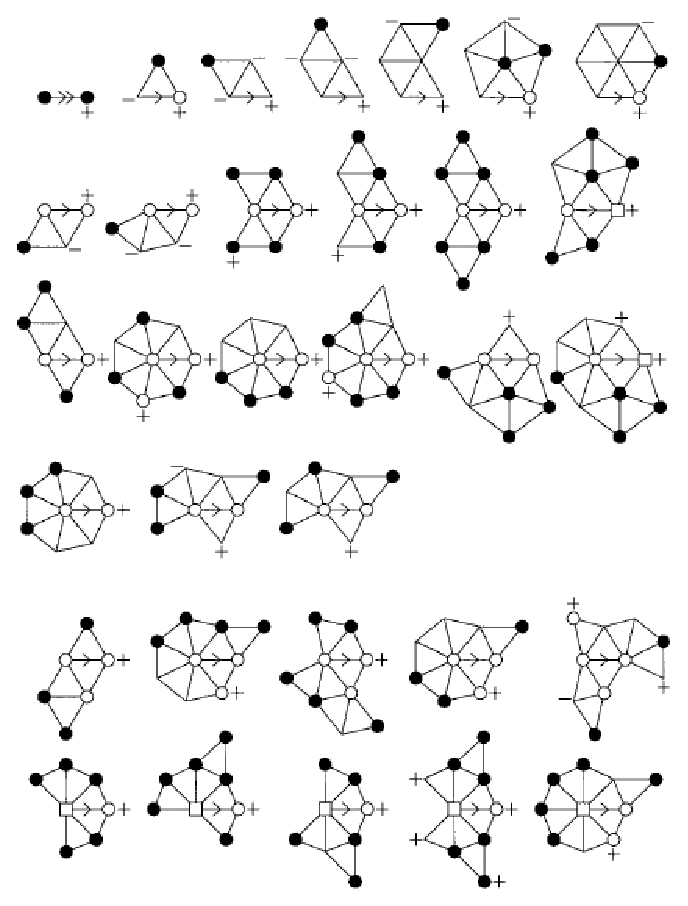
\includegraphics{seymour/regeln.eps}%
  \caption[Darstellung der 32 Regeln]{Darstellung der 32 Regeln, übernommen aus \cite{FourRSST}}
 \end{figure}

 Im weiteren Verlauf dieses Abschnitts benutzen wir $\itP$ nurnoch, um eine Menge von Flüssen zu beschreiben, die einer Regel gehorcht. Dazu ist zu bemerken, dass jeder Fluss genau einer Regel gehorcht, jedoch gibt es für einen Fluss $P$ einige wenige Darstellungen, die einer Regel folgen, deren Isomorphismus von $P$ auf $(K,r,s,t)$ aber nicht eindeutig ist -- zum Beispiel bei den Regeln 10 oder 31. In solchen Fällen zählen wir den Fluss $P$ nur ein mal zu $\itP$, da es sich bei $\itP$ nicht um eine Multimenge handelt.
 
 Flüsse, die der Regel 1 gehorchen, haben den Wert $r=2$, für alle anderen gilt $r=1$. Weiter unterscheiden sich die ersten sieben Regeln von den anderen. Folgt ein Fluss $P$ einer dieser Regeln, so gilt für die Quelle $s$ $\gamma_P(s) \in \{5,6\}$, während in allen anderen Regel für Quelle $s$ und Senke $t$ folgendes gilt: $\gamma_P(s) \in \{7,8\}$ und $\gamma_P(t) \geq 7$. Später werden wir sehen, dass die ersten sieben Regeln einer gewissen Systematik folgen. Alle anderen Regeln wurden jedoch durch stupides Durchprobieren aufgestellt und folgen beim Aufstellen keinem besonderen Muster.
 
 Nun müssen wir noch zeigen, dass unsere Wahl von $\itP$ für Satz \ref{4.4} geeignet ist. Um dies zu erreichen, zerlegen wir Satz \ref{4.4} in drei Fälle, die wir Anhand des Grads der Radnabe $v$ des Wagenrads $W$ unterscheiden:
 \begin{itemize}
  \item $d_W(v) \leq 6$,
  \item $7 \leq d_W(v) \leq 11$ und 
  \item $d_W(v) \geq 12$.
 \end{itemize}
 
 Für den ersten dieser Fälle benötigen wir das folgende Lemma.
 
 \begin{lemmal}{}{4.5}
  Sei $W$ ein Wagenrad mit Radnabe $w$ mit $d_W(w) \in \{5,6\}$. Für $k = 1,\cdots,32$ seien $p_k$ und $q_k$ die Summen über die Werte $r(P)$ aller Flüsse $P$, die der Regel $k$ gehorchen und in $W$ auftreten, bei denen $w$ die Quelle bzw. Senke von $P$ ist. Angenommen, es tritt keine gute Konfiguration in $W$ auf, dann gilt:
  \begin{enumerate}[(i)]
   \item $p_1 = q_2 + q_3$
   \item $p_3 = q_4$
   \item $p_4 = q_5 + q_6$
   \item $p_5 = q_7$
  \end{enumerate}
 \end{lemmal}
 
 \begin{proof}
  Sei $X$ die Menge aller Tripel $(x,y,z)$ von Knoten, die mit $w$ benachbart sind, derart, dass sie alle unterschliedlich sind und $y$ sowohl zu $x$ als auch zu $z$ adjazent ist und $\gamma_W(x) = 5$ gilt. Setze $p_1 = \sharp X$. Sei weiter $q_2$ die Anzahl aller Tripel $(x,y,z) \in X$, für die $\gamma_W(y) \geq 7$ gilt, und $q_3$ die Menge der Tripel $(x,y,z) \in X$ mit $\gamma_W(y) \leq 6$ und $\gamma_W(z) \geq 6$. Da in $W$ nach Voraussetzung keine guten Konfigurationen auftreten, gibt es kein Tripel $(x,y,z) \in X$ mit $\gamma_W(y) \leq 6$ und $\gamma_W(z) = 5$. Somit gilt $q_2 + q_3 = \sharp X = p_1$.\\
  Für den Fall, dass $\gamma_W(w) = 5$ gilt, sind $p_3,p_4,p_5,q_4,q_5,q_6,q_7$ alle 0 und somit (ii), (iii) und (iv) wahr. Im weiteren sei also $\gamma_W(w) = 6$.\\
  Sei nun $X$ die Menge der Tripel $(x,y,z)$ von Knoten, die mit $w$ benachbart sind, derart, dass sie alle unterschliedlich sind, $y$ adjazent zu sowohl $x$ als auch $z$ ist, $\gamma_W(x) \leq 6$, $\gamma_W(y) \leq 6$ und $\gamma_W(u) = 5$ gilt, wobei $u$ der andere Knoten -- nicht $w$ -- ist, der sowohl zu $x$ als auch $y$ adjazent ist. Setze $p_3 = \sharp X$. Da nach Annahme keine gute Konfiguration in $W$ auftritt, gilt für jedes dieser Tripel $\gamma_W(z) \geq 6$. Somit gilt $q_4 = \sharp X = p_3$, was (ii) zeigt.\\
  Die Beweise für (iii) und (iv) verlaufen sehr ähnlich, weswegen hier nicht weiter darauf eingegangen wird.
 \end{proof}

  Aus \ref{4.5} leiten wir Folgendes her.

 \begin{satzl}{gute Konfiguration im Wagenrad I}{4.6}
  Sei $W$ ein Wagenrad mit $N_\itP(W) > 0$ und Radnabe $w$ mit $d_W(w) \in \{5,6\}$. Dann tritt eine gute Konfiguration in $W$ auf.
 \end{satzl}
 
 \begin{proof}
  Seien für die Radnabe $w$ die Werte $p_k$ und $q_k$ definiert für $k = 1,\cdots,32$, genau wie in \ref{4.5}.\\
  Angenommen, es trete keine gute Konfiguration in $W$ auf. Wir werden $N_\itP(W) = 0$ zeigen, was einen Widerspruch darstellt. Sei zuerst $\gamma_W(w) = 5$. Dann sind die $p_k = 0$ für $k = 2,\cdots,32$ und ebenfalls die $q_k = 0$ für $k = 4,\cdots,32$. Somit ergibt sich wegen \ref{4.5}
  \[ N_\itP(W) = 10 + p_1 - q_1 - q_2 - q_3 = 0 \]
  Sei nun $\gamma_W(w) = 6$. Dann folgt wieder aus \ref{4.5}
  \[ N_\itP(W) = p_1 + p_3 + p_4 + p_5 - q_2 - q_3 - q_4 - q_5 - q_6 - q_7 = 0\]
  In beiden Fällen erhalten wir unseren gesuchten Widerspruch durch einfaches Einsetzen.
 \end{proof}
 
 Nun wenden wir uns dem dritten Fall zu, also für Radnaben  mit Grad mindestens $12$. Dafür benötigen wir ein anderes Zwischenresultat.
 
 \begin{lemmal}{}{4.7}
  Sei $W$ ein Wagenrad mit Radnabe $w$ und sei $v$ ein zu $w$ adjazenter Knoten. Wenn keine gute Konfiguration in $W$ auftritt, ist die Summe über die $r(P)$ aller Flüsse $P \in \itP$, die in $W$ auftreten und die Quelle $v$ und Senke $w$ haben, höchstens 5.
 \end{lemmal}

 Der Beweis hierzu verwendet im wesentlichen die Annahme, dass keine gute Konfiguration auftreten darf und betrachtet für jeder der 32 Regeln die Anzahl $R_k$ der Flüsse, die in $W$ auftreten und der $k$-ten Regel folgen, sowie die Summe $R$ aller $R_k$ und zeigt, dass $R \leq 5$ gilt. Dazu unterscheidet er zwischen verschiedenen Zusammensetzungen von $R$ aus den $R_k$ für die fünf verschiedenen Fälle von Werten, di $\gamma_K(v)$ annehmen kann. Dies gestaltet sich sehr lang und trägt wenig zum Verständnis des eigentlichen Problems bei. Deshalb wird für den vollständigen Beweis auf \cite[Seite 21, Lemma 4.7]{FourRSST} verwiesen.
 
 Daraus leiten wir unser nächstes Teilresultat ab.
 
 \begin{satzl}{gute Konfiguration im Wagenrad II}{4.8}
  Sei $W$ ein Wagenrad mit $N_\itP(W) > 0$ und mit Radnabe $w$ mit $d_W(w) \geq 12$. Dann tritt in $W$ eine gute Konfiguration auf.
 \end{satzl}
 
 \begin{proof}
  Angenommen, es würde keine gute Konfiguration in $W$ auftreten. Setze $d = \gamma_W(w)$ und sei $D$ die Menge aller zu $w$ adjazenter Knoten. Für alle $v \in D$ sei $R(v)$ die Summe aller $r(P)$, wobei $P \in \itP$ ein Fluss mit Quelle $v$ und Senke $w$ ist, der in $W$ auftritt. Dann gilt nach \ref{4.7}, dass $\sum_{v \in D} R(v) \leq 5\cdot d$. Somit gilt
  \[ N_\itP(W) = 10(6-d) + \sum_{v \in V} R(v) \leq 10(6-d) + 5d = 60 - 5d \leq 0 \text{,}\]
  was ein Widerspruch ist.
 \end{proof}

 Damit sind zwei der drei Teile unseres ursprünglichen Ziels -- nämlich Satz \ref{4.4} und damit auch Satz \ref{2.3} zu zeigen -- geschafft. Damit bleibt noch die folgende Aussage.

 \begin{satzl}{gute Konfiguration im Wagenrad III}{4.9}
  Sei $W$ ein Wagenrad mit $N_\itP(W) > 0$ und mit Radnabe $w$ mit $d_W(w) \in \{7,8,9,10,11\}$. Dann tritt in $W$ eine gute Konfiguration auf.
 \end{satzl}
 
 Diesen wesentlichen Schritt führten \rsst\-\ in voller Länge aus -- insgesamt etwa 13000 Zeilen. Dazu verfassten sie den Beweis in maschinenlesbarer Form, die von Hand nachprüfbar ist. Dieses Nachprüfen ist zumindest theoretisch möglich, jedoch raten die vier Authoren wegen der schieren Länge davon ab. Stattdessen empfehlen sie, die Korrektheit des angegebenen Beweisalgorithmus mit einem anderen Computerprogramm zu verifizieren, was bereits nach damaligem Stand der Technick innerhalb weniger Minuten möglich war.

 Kombiniert man nun die Sätze \ref{4.6}, \ref{4.8} und \ref{4.9}, so erhält man die Aussage \ref{4.4}. Daraus ergibt sich dann die Korrektheit der Aussage \ref{2.3}, die diesen Abschnitt motiviert hat.



\end{section}
\end{chapter}
